%
% content.tex -- Buch zum mathematischen Seminar Harmonische Analysis
%
% (c) 2023 Prof. Dr. Andreas Mueller, OST Ostschweizer Fachhochschule
%
% TODO: Platziere dieses Dokument auf der gleichen Ebene wie buch.tex
\def\IncludeBookCover{0}
\documentclass{book}
%
% packages.tex -- special packages needed by doppelpendel
%


% additional packages used by the individual papers, add a line for
% each paper
%
% addpackages.tex -- file to add all paper packages files
%
% (c) 2023 Prof Dr Andreas Müller, OST Ostschweizer Fachhochschule
%
%
% packages.tex -- special packages needed by doppelpendel
%



% PDF info
\hypersetup{
pdftitle={Mathematisches Seminar Variationsprinzipien},
pdfauthor={Andreas Müller}
}

% workaround for biblatex bug
\makeatletter
\def\blx@maxline{77}
\makeatother
\addbibresource{chapters/references.bib}

% Bibresources for each article
\addbibresource{papers/relativ/references.bib} % TODO: Link zu deinem Literaturverzeichnis
% %
% addbibresources.tex -- file to add all bib resources
%
% (c) 2020 Prof Dr Andreas Müller, Hochschule Rapperswil
%
\addbibresource{../papers/doppelpendel/references.bib}
\addbibresource{../papers/kettenlinie/references.bib}
\addbibresource{../papers/balken/references.bib}
\addbibresource{../papers/relativ/references.bib}
\addbibresource{../papers/maxwell/references.bib}
\addbibresource{../papers/geodaeten/references.bib}
\addbibresource{../papers/minimalflaechen/references.bib}
\addbibresource{../papers/leo/references.bib}
\addbibresource{../papers/circuit/references.bib}
\addbibresource{../papers/antennen/references.bib}
\addbibresource{../papers/fem/references.bib}
\addbibresource{../papers/schwimmen/references.bib}
\addbibresource{../papers/planet/references.bib}
\addbibresource{../papers/varalg/references.bib}
\addbibresource{../papers/cahnhilliard/references.bib}
\addbibresource{../papers/luke/references.bib}
\addbibresource{../papers/variationsprinzip_algorithmen/references.bib}
\addbibresource{../papers/widerstand/references.bib}


% make sure the last index starts on an odd page
\AtEndDocument{\clearpage\ifodd\value{page}\else\null\clearpage\fi}
\makeindex

%\pgfplotsset{compat=1.12}
\setlength{\headheight}{15pt} % fix headheight warning
\DeclareGraphicsRule{*}{mps}{*}{}
\begin{document}

% cover page
\ifthenelse{\boolean{includecover}}{
\incgraph[documentpaper][width=\paperwidth,height=\paperheight]{cover/buchcover.jpg}
\newpage\null\thispagestyle{empty}\newpage
}{}

\input{common/titlepage.tex}

% add common macros
\input{common/macros.tex}

\mainmatter

%
% part2.tex -- format the second part
%
\part{Anwendungen und weiterführende Themen}
\fancyhead[RE]{Anwendungen}
\fancyhead[LO]{Anwendungen}
\def\chapterauthor#1{{\large #1}\bigskip\bigskip}
%
% main.tex -- Paper zum Thema <schwimmen>
%
% (c) 2020 Autor, OST Ostschweizer Fachhochschule
%
% !TEX root = ../../buch.tex
% !TEX encoding = UTF-8
%
\chapter{Die Optimale Flussüberquerung\label{chapter:schwimmen}}
\kopflinks{Thema}
\begin{refsection}
	\chapterauthor{Anna Pietak}
	
	
	Das Überqueren eines Flusses ist seit jeher eine Herausforderung, die die Menschheit seit Anbeginn beschäftigt. Oft auch im Zusammenhang mit der Frage, wie man am besten mit einem Boot einen Fluss überquert, sind vielfältige Überlegungen angestellt worden. Einige einfache Ansätze könnten darin bestehen, den Fluss an einer flachen Stelle zu überqueren, wo man zu Fuss hindurch waten kann, oder ihn einfach gemütlich schwimmend zu durchqueren und einfach in kauf nehmen das die Strömung einen mitreisst.
	
	
	Die zentrale Frage, die sich hier stellt, ist jedoch: Wie überquere ich einen Fluss am energieeffizientesten? In Abbildung \ref{fig:river_original} ist ein solcher Fluss dargestellt, der überquert werden soll.
	
	
	
	
	\begin{figure}
		\centering
		\tikzset{every picture/.style={line width=0.75pt}} %set default line width to 0.75pt        
		
		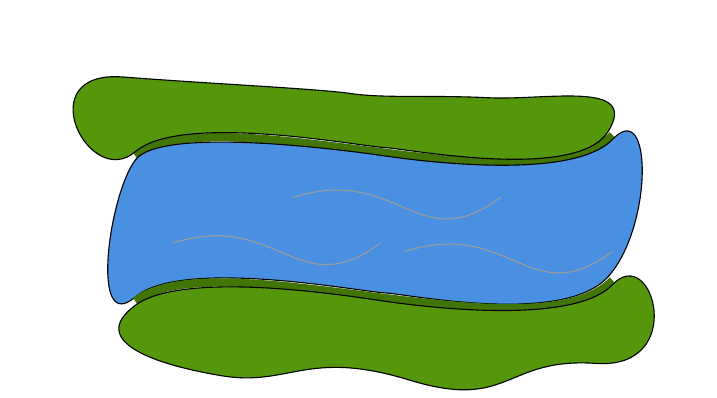
\begin{tikzpicture}[x=0.75pt,y=0.75pt,yscale=-1,xscale=1]
			%uncomment if require: \path (0,300); %set diagram left start at 0, and has height of 300
			
			%Curve Lines [id:da608977851192717] 
			\draw [color={rgb, 255:red, 65; green, 117; blue, 5 }  ,draw opacity=1 ][line width=3]    (300,110) .. controls (340,80) and (493.51,138.06) .. (530,100) ;
			%Shape: Polygon Curved [id:ds9392726871646548] 
			\draw  [fill={rgb, 255:red, 74; green, 144; blue, 226 }  ,fill opacity=1 ] (300,112) .. controls (312.68,95.2) and (403.92,107.66) .. (420,110) .. controls (436.08,112.34) and (510.65,122.34) .. (530,102) .. controls (549.35,81.66) and (549.3,143.91) .. (528,168) .. controls (506.7,192.09) and (432.13,176.66) .. (420,176) .. controls (407.87,175.34) and (322.13,158.94) .. (300,178) .. controls (277.87,197.06) and (287.32,128.8) .. (300,112) -- cycle ;
			%Curve Lines [id:da6433547723995421] 
			\draw [color={rgb, 255:red, 65; green, 117; blue, 5 }  ,draw opacity=1 ][line width=3]    (300,180) .. controls (340,150) and (493.51,208.06) .. (530,170) ;
			%Shape: Polygon Curved [id:ds34371397326569686] 
			\draw  [fill={rgb, 255:red, 85; green, 151; blue, 11 }  ,fill opacity=1 ] (300,182) .. controls (323.56,164.66) and (403.92,177.66) .. (420,180) .. controls (436.08,182.34) and (510.65,192.34) .. (530,172) .. controls (549.35,151.66) and (566.44,213.06) .. (522,210) .. controls (477.56,206.94) and (481.01,233.06) .. (432,218) .. controls (382.99,202.94) and (374.13,221.23) .. (342,216) .. controls (309.87,210.77) and (276.44,199.34) .. (300,182) -- cycle ;
			%Shape: Polygon Curved [id:ds3342416894164969] 
			\draw  [fill={rgb, 255:red, 85; green, 151; blue, 11 }  ,fill opacity=1 ] (294,72) .. controls (339.58,75.49) and (387.92,77.66) .. (404,80) .. controls (420.08,82.34) and (442.15,80.63) .. (470,82) .. controls (497.85,83.37) and (542.72,73.49) .. (528,98) .. controls (513.28,122.51) and (432.13,106.66) .. (420,106) .. controls (407.87,105.34) and (322.13,88.94) .. (300,108) .. controls (277.87,127.06) and (248.42,68.51) .. (294,72) -- cycle ;
			%Curve Lines [id:da7504908272245701] 
			\draw [color={rgb, 255:red, 155; green, 155; blue, 155 }  ,draw opacity=1 ]   (318,152) .. controls (369.01,135.91) and (378,182) .. (418,152) ;
			%Curve Lines [id:da01966435364089625] 
			\draw [color={rgb, 255:red, 155; green, 155; blue, 155 }  ,draw opacity=1 ]   (376,130) .. controls (427.01,113.91) and (436,160) .. (476,130) ;
			%Curve Lines [id:da5498107083025197] 
			\draw [color={rgb, 255:red, 155; green, 155; blue, 155 }  ,draw opacity=1 ]   (430,156) .. controls (481.01,139.91) and (490,186) .. (530,156) ;
			
			
			
			
		\end{tikzpicture}
		
		\caption{Fluss der überquert werden soll. Blau ist der Fluss eingezeichnet und grün das Ufer.}
		\label{fig:river_original}
	\end{figure}
	
	Für die Frage \textit{Wie schwimmt man am besten durch den Fluss?} wird zudem vorausgesetzt, dass das Ziel auf derselben Höhe auf der anderen Seite des Flusses erreicht werden soll. Was bedeutet das man die ganze Strömung durch flussaufwärs schwimmen kompensiert werden muss. Dies ist in Abbildung \ref{fig:river_points} veranschaulicht. Die Frage, die uns hier beschäftigt, lautet: Wie schwimmt man am besten von Punkt A nach Punkt B?
	
	
	
	
	
	
	\begin{figure}
		\centering
		
		
		\tikzset{every picture/.style={line width=0.75pt}} %set default line width to 0.75pt        
		
		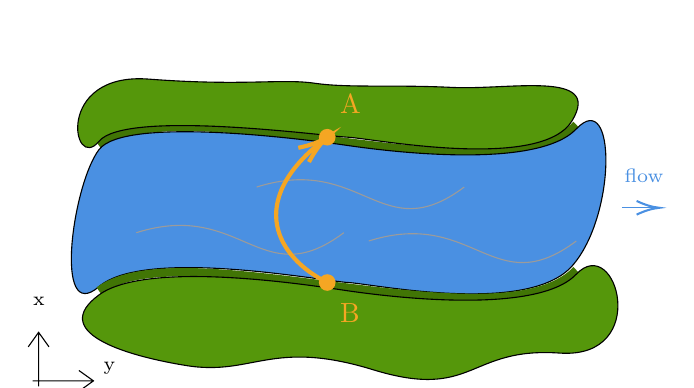
\begin{tikzpicture}[x=0.75pt,y=0.75pt,yscale=-1,xscale=1]
			%uncomment if require: \path (0,300); %set diagram left start at 0, and has height of 300
			
			%Curve Lines [id:da608977851192717] 
			\draw [color={rgb, 255:red, 65; green, 117; blue, 5 }  ,draw opacity=1 ][line width=3]    (300,110) .. controls (340,80) and (493.51,138.06) .. (530,100) ;
			%Shape: Polygon Curved [id:ds9392726871646548] 
			\draw  [fill={rgb, 255:red, 74; green, 144; blue, 226 }  ,fill opacity=1 ] (300,112) .. controls (312.68,95.2) and (403.92,107.66) .. (420,110) .. controls (436.08,112.34) and (510.65,122.34) .. (530,102) .. controls (549.35,81.66) and (549.3,143.91) .. (528,168) .. controls (506.7,192.09) and (432.13,176.66) .. (420,176) .. controls (407.87,175.34) and (322.13,158.94) .. (300,178) .. controls (277.87,197.06) and (287.32,128.8) .. (300,112) -- cycle ;
			%Curve Lines [id:da6433547723995421] 
			\draw [color={rgb, 255:red, 65; green, 117; blue, 5 }  ,draw opacity=1 ][line width=3]    (300,180) .. controls (340,150) and (493.51,208.06) .. (530,170) ;
			%Shape: Polygon Curved [id:ds34371397326569686] 
			\draw  [fill={rgb, 255:red, 85; green, 151; blue, 11 }  ,fill opacity=1 ] (300,182) .. controls (323.56,164.66) and (403.92,177.66) .. (420,180) .. controls (436.08,182.34) and (510.65,192.34) .. (530,172) .. controls (549.35,151.66) and (566.44,213.06) .. (522,210) .. controls (477.56,206.94) and (481.01,233.06) .. (432,218) .. controls (382.99,202.94) and (374.13,221.23) .. (342,216) .. controls (309.87,210.77) and (276.44,199.34) .. (300,182) -- cycle ;
			%Shape: Polygon Curved [id:ds3342416894164969] 
			\draw  [fill={rgb, 255:red, 85; green, 151; blue, 11 }  ,fill opacity=1 ] (324,78) .. controls (369.58,81.49) and (387.92,77.66) .. (404,80) .. controls (420.08,82.34) and (442.15,80.63) .. (470,82) .. controls (497.85,83.37) and (542.72,73.49) .. (528,98) .. controls (513.28,122.51) and (432.13,106.66) .. (420,106) .. controls (407.87,105.34) and (312.7,92.51) .. (300,108) .. controls (287.3,123.49) and (278.42,74.51) .. (324,78) -- cycle ;
			%Curve Lines [id:da7504908272245701] 
			\draw [color={rgb, 255:red, 155; green, 155; blue, 155 }  ,draw opacity=1 ]   (318,152) .. controls (369.01,135.91) and (378,182) .. (418,152) ;
			%Curve Lines [id:da01966435364089625] 
			\draw [color={rgb, 255:red, 155; green, 155; blue, 155 }  ,draw opacity=1 ]   (376,130) .. controls (427.01,113.91) and (436,160) .. (476,130) ;
			%Curve Lines [id:da5498107083025197] 
			\draw [color={rgb, 255:red, 155; green, 155; blue, 155 }  ,draw opacity=1 ]   (430,156) .. controls (481.01,139.91) and (490,186) .. (530,156) ;
			%Shape: Circle [id:dp01198373160385724] 
			\draw  [draw opacity=0][fill={rgb, 255:red, 245; green, 166; blue, 35 }  ,fill opacity=1 ] (406,106) .. controls (406,103.79) and (407.79,102) .. (410,102) .. controls (412.21,102) and (414,103.79) .. (414,106) .. controls (414,108.21) and (412.21,110) .. (410,110) .. controls (407.79,110) and (406,108.21) .. (406,106) -- cycle ;
			%Shape: Circle [id:dp6252725126232461] 
			\draw  [draw opacity=0][fill={rgb, 255:red, 245; green, 166; blue, 35 }  ,fill opacity=1 ] (406,176) .. controls (406,173.79) and (407.79,172) .. (410,172) .. controls (412.21,172) and (414,173.79) .. (414,176) .. controls (414,178.21) and (412.21,180) .. (410,180) .. controls (407.79,180) and (406,178.21) .. (406,176) -- cycle ;
			%Straight Lines [id:da006269855405936053] 
			\draw [color={rgb, 255:red, 74; green, 144; blue, 226 }  ,draw opacity=1 ]   (552,140) -- (568,140) ;
			\draw [shift={(570,140)}, rotate = 180] [color={rgb, 255:red, 74; green, 144; blue, 226 }  ,draw opacity=1 ][line width=0.75]    (10.93,-3.29) .. controls (6.95,-1.4) and (3.31,-0.3) .. (0,0) .. controls (3.31,0.3) and (6.95,1.4) .. (10.93,3.29)   ;
			%Shape: Axis 2D [id:dp579588107341299] 
			\draw  (268,223.4) -- (297.36,223.4)(270.94,200) -- (270.94,226) (290.36,218.4) -- (297.36,223.4) -- (290.36,228.4) (265.94,207) -- (270.94,200) -- (275.94,207)  ;
			%Curve Lines [id:da1687299064997403] 
			\draw [color={rgb, 255:red, 245; green, 166; blue, 35 }  ,draw opacity=1 ][line width=1.5]    (410,176) .. controls (385.7,163.93) and (370.61,137.1) .. (407.67,107.8) ;
			\draw [shift={(410,106)}, rotate = 143.13] [color={rgb, 255:red, 245; green, 166; blue, 35 }  ,draw opacity=1 ][line width=1.5]    (14.21,-4.28) .. controls (9.04,-1.82) and (4.3,-0.39) .. (0,0) .. controls (4.3,0.39) and (9.04,1.82) .. (14.21,4.28)   ;
			
			% Text Node
			\draw (415,84) node [anchor=north west][inner sep=0.75pt]  [color={rgb, 255:red, 245; green, 166; blue, 35 }  ,opacity=1 ] [align=left] {A};
			% Text Node
			\draw (415,185) node [anchor=north west][inner sep=0.75pt]  [color={rgb, 255:red, 245; green, 166; blue, 35 }  ,opacity=1 ] [align=left] {B};
			% Text Node
			\draw (552,120) node [anchor=north west][inner sep=0.75pt]  [color={rgb, 255:red, 74; green, 144; blue, 226 }  ,opacity=1 ] [align=left] {{\scriptsize flow}};
			% Text Node
			\draw (267,182) node [anchor=north west][inner sep=0.75pt]  [color={rgb, 255:red, 0; green, 0; blue, 0 }  ,opacity=1 ] [align=left] {{\scriptsize x}};
			% Text Node
			\draw (301,213) node [anchor=north west][inner sep=0.75pt]  [color={rgb, 255:red, 0; green, 0; blue, 0 }  ,opacity=1 ] [align=left] {{\scriptsize y}};
			
			
		\end{tikzpicture}
		
		
		\caption{Fluss der überquert werden soll. Blau ist der Fluss eingezeichnet und grün das Ufer. Die Strömung geht von liks nach rechts und ist mit dem Pfeil eingezeichnet. Unten links noch ein referenz kordinaten System.}
		\label{fig:river_points}
	\end{figure}
	
	In diesem Kapitel wird erläutert, wie man mittels des Variationsprinzips die optimale Schwimmroute über den Fluss findet.
	
	
	
	
	
	
	% Ein paar Hinweise für die korrekte Formatierung des Textes
	% \begin{itemize}
		% \item
		% Absätze werden gebildet, indem man eine Leerzeile einfügt.
		% Die Verwendung von \verb+\\+ ist nur in Tabellen und Arrays gestattet.
		% \item
		% Die explizite Platzierung von Bildern ist nicht erlaubt, entsprechende
		% Optionen werden gelöscht. 
		% Verwenden Sie Labels und Verweise, um auf Bilder hinzuweisen.
		% \item
		% Beginnen Sie jeden Satz auf einer neuen Zeile. 
		% Damit ermöglichen Sie dem Versionsverwaltungssysteme, Änderungen
		% in verschiedenen Sätzen von verschiedenen Autoren ohne Konflikt 
		% anzuwenden.
		% \item 
		% Bilden Sie auch für Formeln kurze Zeilen, einerseits der besseren
		% Übersicht wegen, aber auch um GIT die Arbeit zu erleichtern.
		% \end{itemize}


%
% einleitung.tex -- Beispiel-File für die Einleitung
%
% (c) 2020 Prof Dr Andreas Müller, Hochschule Rapperswil
%
% !TEX root = ../../buch.tex
% !TEX encoding = UTF-8
%
\section{Herangehensweise\label{schwimmen:section:teil0}}
\rhead{Herangehensweise}

Es soll ermittelt werden, welche die energieeffizienteste Methode ist, um den Fluss zu überqueren. Da die Energie \(E\) mittels der Formel \[E = P \cdot t\] berechnet werden kann, wobei \(P\) für die Leistung und \(t\) für die Zeit steht, stellt sich heraus, dass die Energie für die Flussüberquerung direkt von der Zeit abhängt. Ergo sollte es möglich sein, nicht die Energie zu optimieren, sondern die Zeit.

Dies vereinfacht vieles, allerdings muss nun die Leistung, mit der geschwommen werden kann, begrenzt werden. Eine schwimmende Person kann nicht unbegrenzt schnell schwimmen und somit nicht in keiner Zeit am anderen Ufer ankommen.

\subsection{Variationsprinzip}
Das Variationsprinzip ist ein Konzept, das besagt, dass die Natur in vielen Fällen den optimalen Weg wählt. In diesem Fall ist es das Prinzip der kleinsten Wirkung, also des kleinsten Energieaufwand, der für die Flussüberquerung benötigt wird. Die Euler-Lagrange-Differentialgleichung ist das Werkzeug, um das Variationsprinzip zu berechnen. Das Lagrange-Integral gibt das Minimum der Wirkung zurück.



% Es soll ermitelt werden was die energieefizientiste Methode ist um den Fluss zu überqueren. Da die Energie \(E\) mittels der Formel \[E=P\cdot t\] berechnet werden kann wobei \(P\) für die Leistung und \(t\) für die Zeit steht, stehlt sich heraus das die Energie für die Flussüberquerung direkt von der Zeit abhängig ist. Ergo sollte es möglich sein nicht eine Optimierung der Energie sondern eine der Zeit zu machen. 
% Das vereinfacht vieles, jetzt muss man aber die Leistung mit der man schwimmen kann beschränken. Die schwimmende Person kann nicht unbeschränkt schnell schwimmen und dadurch in keiner Zeit am anderen Ufer ankommen.

% \subsection{Variationsprinzip}
% Das Variationsprinzip ist ein Konzept, das besagt, dass die Natur in vielen Fällen den optimalen Weg wählt. In diesem Fall ist es das Prinzip der kleinsten Wrikung, der kleinste Energieaufwand der für die Flussüberquerung gebraucht wird.
% Die Lagrange Formel ist das Werkzueg um das Variationsprinzip zu berechnen. Das Lagrange-Integral gibt das minimum der Wirkung zurück.









% Lorem ipsum dolor sit amet, consetetur sadipscing elitr, sed diam
% nonumy eirmod tempor invidunt ut labore et dolore magna aliquyam
% erat, sed diam voluptua \cite{schwimmen:bibtex}.
% At vero eos et accusam et justo duo dolores et ea rebum.
% Stet clita kasd gubergren, no sea takimata sanctus est Lorem ipsum
% dolor sit amet.

% Lorem ipsum dolor sit amet, consetetur sadipscing elitr, sed diam
% nonumy eirmod tempor invidunt ut labore et dolore magna aliquyam
% erat, sed diam voluptua.
% At vero eos et accusam et justo duo dolores et ea rebum.  Stet clita
% kasd gubergren, no sea takimata sanctus est Lorem ipsum dolor sit
% amet.



%
% teil1.tex -- Beispiel-File für das Paper
%
% (c) 2020 Prof Dr Andreas Müller, Hochschule Rapperswil
%
% !TEX root = ../../buch.tex
% !TEX encoding = UTF-8
%
\section{Naiver Weg
\label{schwimmen:section:naiver_weg}}
\rhead{Problemstellung}



\begin{figure}
    \centering
       
   

    \tikzset{every picture/.style={line width=0.75pt}} %set default line width to 0.75pt        
    
    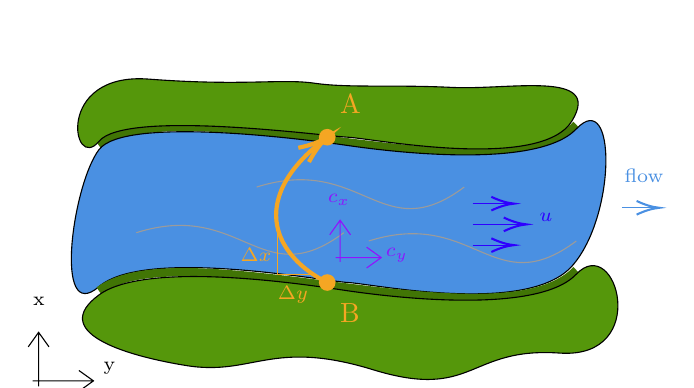
\begin{tikzpicture}[x=0.75pt,y=0.75pt,yscale=-1,xscale=1]
%uncomment if require: \path (0,300); %set diagram left start at 0, and has height of 300

%Curve Lines [id:da608977851192717] 
\draw [color={rgb, 255:red, 65; green, 117; blue, 5 }  ,draw opacity=1 ][line width=3]    (300,110) .. controls (340,80) and (493.51,138.06) .. (530,100) ;
%Shape: Polygon Curved [id:ds9392726871646548] 
\draw  [fill={rgb, 255:red, 74; green, 144; blue, 226 }  ,fill opacity=1 ] (300,112) .. controls (312.68,95.2) and (403.92,107.66) .. (420,110) .. controls (436.08,112.34) and (510.65,122.34) .. (530,102) .. controls (549.35,81.66) and (549.3,143.91) .. (528,168) .. controls (506.7,192.09) and (432.13,176.66) .. (420,176) .. controls (407.87,175.34) and (322.13,158.94) .. (300,178) .. controls (277.87,197.06) and (287.32,128.8) .. (300,112) -- cycle ;
%Curve Lines [id:da6433547723995421] 
\draw [color={rgb, 255:red, 65; green, 117; blue, 5 }  ,draw opacity=1 ][line width=3]    (300,180) .. controls (340,150) and (493.51,208.06) .. (530,170) ;
%Shape: Polygon Curved [id:ds34371397326569686] 
\draw  [fill={rgb, 255:red, 85; green, 151; blue, 11 }  ,fill opacity=1 ] (300,182) .. controls (323.56,164.66) and (403.92,177.66) .. (420,180) .. controls (436.08,182.34) and (510.65,192.34) .. (530,172) .. controls (549.35,151.66) and (566.44,213.06) .. (522,210) .. controls (477.56,206.94) and (481.01,233.06) .. (432,218) .. controls (382.99,202.94) and (374.13,221.23) .. (342,216) .. controls (309.87,210.77) and (276.44,199.34) .. (300,182) -- cycle ;
%Shape: Polygon Curved [id:ds3342416894164969] 
\draw  [fill={rgb, 255:red, 85; green, 151; blue, 11 }  ,fill opacity=1 ] (324,78) .. controls (369.58,81.49) and (387.92,77.66) .. (404,80) .. controls (420.08,82.34) and (442.15,80.63) .. (470,82) .. controls (497.85,83.37) and (542.72,73.49) .. (528,98) .. controls (513.28,122.51) and (432.13,106.66) .. (420,106) .. controls (407.87,105.34) and (312.7,92.51) .. (300,108) .. controls (287.3,123.49) and (278.42,74.51) .. (324,78) -- cycle ;
%Curve Lines [id:da7504908272245701] 
\draw [color={rgb, 255:red, 155; green, 155; blue, 155 }  ,draw opacity=1 ]   (318,152) .. controls (369.01,135.91) and (378,182) .. (418,152) ;
%Curve Lines [id:da01966435364089625] 
\draw [color={rgb, 255:red, 155; green, 155; blue, 155 }  ,draw opacity=1 ]   (376,130) .. controls (427.01,113.91) and (436,160) .. (476,130) ;
%Curve Lines [id:da5498107083025197] 
\draw [color={rgb, 255:red, 155; green, 155; blue, 155 }  ,draw opacity=1 ]   (430,156) .. controls (481.01,139.91) and (490,186) .. (530,156) ;
%Shape: Circle [id:dp01198373160385724] 
\draw  [draw opacity=0][fill={rgb, 255:red, 245; green, 166; blue, 35 }  ,fill opacity=1 ] (406,106) .. controls (406,103.79) and (407.79,102) .. (410,102) .. controls (412.21,102) and (414,103.79) .. (414,106) .. controls (414,108.21) and (412.21,110) .. (410,110) .. controls (407.79,110) and (406,108.21) .. (406,106) -- cycle ;
%Shape: Circle [id:dp6252725126232461] 
\draw  [draw opacity=0][fill={rgb, 255:red, 245; green, 166; blue, 35 }  ,fill opacity=1 ] (406,176) .. controls (406,173.79) and (407.79,172) .. (410,172) .. controls (412.21,172) and (414,173.79) .. (414,176) .. controls (414,178.21) and (412.21,180) .. (410,180) .. controls (407.79,180) and (406,178.21) .. (406,176) -- cycle ;
%Straight Lines [id:da006269855405936053] 
\draw [color={rgb, 255:red, 74; green, 144; blue, 226 }  ,draw opacity=1 ]   (552,140) -- (568,140) ;
\draw [shift={(570,140)}, rotate = 180] [color={rgb, 255:red, 74; green, 144; blue, 226 }  ,draw opacity=1 ][line width=0.75]    (10.93,-3.29) .. controls (6.95,-1.4) and (3.31,-0.3) .. (0,0) .. controls (3.31,0.3) and (6.95,1.4) .. (10.93,3.29)   ;
%Shape: Axis 2D [id:dp579588107341299] 
\draw  (268,223.4) -- (297.36,223.4)(270.94,200) -- (270.94,226) (290.36,218.4) -- (297.36,223.4) -- (290.36,228.4) (265.94,207) -- (270.94,200) -- (275.94,207)  ;
%Curve Lines [id:da1687299064997403] 
\draw [color={rgb, 255:red, 245; green, 166; blue, 35 }  ,draw opacity=1 ][line width=1.5]    (410,176) .. controls (385.7,163.93) and (370.61,137.1) .. (407.67,107.8) ;
\draw [shift={(410,106)}, rotate = 143.13] [color={rgb, 255:red, 245; green, 166; blue, 35 }  ,draw opacity=1 ][line width=1.5]    (14.21,-4.28) .. controls (9.04,-1.82) and (4.3,-0.39) .. (0,0) .. controls (4.3,0.39) and (9.04,1.82) .. (14.21,4.28)   ;
%Straight Lines [id:da5117559499291524] 
\draw [color={rgb, 255:red, 245; green, 166; blue, 35 }  ,draw opacity=1 ]   (386,146) -- (386,172) ;
%Straight Lines [id:da7911427218260162] 
\draw [color={rgb, 255:red, 245; green, 166; blue, 35 }  ,draw opacity=1 ]   (386,172) -- (404,172) ;
%Shape: Axis 2D [id:dp020929963075495994] 
\draw [color={rgb, 255:red, 144; green, 19; blue, 254 }  ,draw opacity=1 ] (414,164) -- (436,164)(416.2,146) -- (416.2,166) (429,159) -- (436,164) -- (429,169) (411.2,153) -- (416.2,146) -- (421.2,153)  ;
%Straight Lines [id:da5963450198567739] 
\draw [color={rgb, 255:red, 46; green, 0; blue, 255 }  ,draw opacity=1 ]   (480,148) -- (504,148) ;
\draw [shift={(506,148)}, rotate = 180] [color={rgb, 255:red, 46; green, 0; blue, 255 }  ,draw opacity=1 ][line width=0.75]    (10.93,-3.29) .. controls (6.95,-1.4) and (3.31,-0.3) .. (0,0) .. controls (3.31,0.3) and (6.95,1.4) .. (10.93,3.29)   ;
%Straight Lines [id:da016477493607424232] 
\draw [color={rgb, 255:red, 46; green, 0; blue, 255 }  ,draw opacity=1 ]   (480,158) -- (498,158) ;
\draw [shift={(500,158)}, rotate = 180] [color={rgb, 255:red, 46; green, 0; blue, 255 }  ,draw opacity=1 ][line width=0.75]    (10.93,-3.29) .. controls (6.95,-1.4) and (3.31,-0.3) .. (0,0) .. controls (3.31,0.3) and (6.95,1.4) .. (10.93,3.29)   ;
%Straight Lines [id:da8245950958515168] 
\draw [color={rgb, 255:red, 46; green, 0; blue, 255 }  ,draw opacity=1 ]   (480,138) -- (498,138) ;
\draw [shift={(500,138)}, rotate = 180] [color={rgb, 255:red, 46; green, 0; blue, 255 }  ,draw opacity=1 ][line width=0.75]    (10.93,-3.29) .. controls (6.95,-1.4) and (3.31,-0.3) .. (0,0) .. controls (3.31,0.3) and (6.95,1.4) .. (10.93,3.29)   ;

% Text Node
\draw (415,84) node [anchor=north west][inner sep=0.75pt]  [color={rgb, 255:red, 245; green, 166; blue, 35 }  ,opacity=1 ] [align=left] {A};
% Text Node
\draw (415,185) node [anchor=north west][inner sep=0.75pt]  [color={rgb, 255:red, 245; green, 166; blue, 35 }  ,opacity=1 ] [align=left] {B};
% Text Node
\draw (552,120) node [anchor=north west][inner sep=0.75pt]  [color={rgb, 255:red, 74; green, 144; blue, 226 }  ,opacity=1 ] [align=left] {{\scriptsize flow}};
% Text Node
\draw (267,182) node [anchor=north west][inner sep=0.75pt]  [color={rgb, 255:red, 0; green, 0; blue, 0 }  ,opacity=1 ] [align=left] {{\scriptsize x}};
% Text Node
\draw (301,213) node [anchor=north west][inner sep=0.75pt]  [color={rgb, 255:red, 0; green, 0; blue, 0 }  ,opacity=1 ] [align=left] {{\scriptsize y}};
% Text Node
\draw (385,176.4) node [anchor=north west][inner sep=0.75pt]  [font=\scriptsize]  {$\textcolor[rgb]{0.96,0.65,0.14}{\Delta y}$};
% Text Node
\draw (367,158.4) node [anchor=north west][inner sep=0.75pt]  [font=\scriptsize]  {$\textcolor[rgb]{0.96,0.65,0.14}{\Delta x}$};
% Text Node
\draw (409,132.4) node [anchor=north west][inner sep=0.75pt]  [font=\scriptsize,color={rgb, 255:red, 144; green, 19; blue, 254 }  ,opacity=1 ]  {$\textcolor[rgb]{0.56,0.07,1}{c_{x}}$};
% Text Node
\draw (437,158.4) node [anchor=north west][inner sep=0.75pt]  [font=\scriptsize,color={rgb, 255:red, 144; green, 19; blue, 254 }  ,opacity=1 ]  {$\textcolor[rgb]{0.56,0.07,1}{c_{y}}$};
% Text Node
\draw (511,141.4) node [anchor=north west][inner sep=0.75pt]  [font=\scriptsize,color={rgb, 255:red, 144; green, 19; blue, 254 }  ,opacity=1 ]  {$\textcolor[rgb]{0.18,0,1}{u}$};


\end{tikzpicture}



    \caption{Fluss, der überquert werden soll. Die Strömungsgeschwindigkeit \(u\) ist dunkelblau eingezeichnet und bezieht sich auf die Geschwindigkeit des Flusses. Dabei ist zu beachten, dass diese nicht überall im Fluss gleich sein muss; sie könnte zum Ufer hin langsamer und in der Mitte des Flusses schneller sein. Somit ist sie von \(x\) abhängig. \(c_x\) und \(c_y\) bezeichnen die Geschwindigkeiten in \(x\)- und \(y\)-Richtung der schwimmenden Person. \(\Delta x\) und \(\Delta y\) sind die sehr kleinen Distanzen auf der Strecke von A nach B.
    \label{fig:river_dif}}
\end{figure}

\textbf{Zeitoptimierung} Die Zeit \(T\), die für die Flussüberquerung benötigt wird, kann mittels
\[
T = \int \frac{1}{v} \, ds
\]
berechnet werden, wobei \(v\) die Geschwindigkeit ist und \(s\) die dabei zurückgelegte Strecke.

\textbf{Zeit für ein Streckenstück} Die Zeit, die für ein sehr kleines Streckenstück benötigt wird, kann ermittelt werden, indem man diese kleine Strecke durch die Geschwindigkeit auf dieser kleinen Strecke teilt. Dies sieht so aus:
\begin{equation}\label{eq:time_for_distance_pice}
    \frac{ds}{\sqrt{(c_y - u)^2 + c_x^2}}
\end{equation}
wobei \(u\) die Geschwindigkeit des Flusses bzw. der Strömung an dieser Stelle im Fluss ist. \(c_x\) und \(c_y\) bezeichnen die Geschwindigkeiten der schwimmenden Person in \(x\)- und \(y\)-Richtung. Eine grafische Darstellung ist in Abbildung \ref{fig:river_dif} zu sehen.

\textbf{Zeit für die Strömungskompensation} Die Zeit, die zusätzlich zur Flussüberquerung benötigt wird, um die Strömung zu kompensieren, ist definiert als 
\begin{equation}\label{eq:time_compenation}
    \frac{dx}{u}
\end{equation}

\textbf{Gesamte Zeit} Die gesamte Zeit für ein sehr kleines Streckenstück kann mittels der Gleichungen \ref{eq:time_for_distance_pice} und \ref{eq:time_compenation} hergeleitet werden. Es folgt:
\begin{equation}\label{eq:time_pice_total}
    \frac{dx}{u} + \frac{ds}{\sqrt{(c_y - u)^2 + c_x^2}}
\end{equation}

\textbf{Strecke}
Für allgemeine Fälle kann die Distanz einer Strecke mit der Formel
\[
ds = \sqrt{\Delta x^2 + \Delta y^2} \approx \sqrt{1 + y'^2} \, dx
\]
angenähert werden, wobei sich die Variablen wieder auf Abbildung \ref{fig:river_dif} beziehen.

\textbf{Integral} Nun ist es an der Zeit, ein Integral für die Zeit, die benötigt wird, um den Fluss zu überqueren, aufzustellen, basierend auf den obigen Formeln. Das Integral:
\begin{equation}\label{eq:integral_time}
    T = \int L(x, y, y') \, dx = \int \left( \frac{1}{u} + \frac{\sqrt{1 + y'^2}}{\sqrt{(c_y - u)^2 + c_x^2}} \right) dx
\end{equation}
soll für eine möglichst kleine Zeit \(T\) optimiert werden, um die energieeffizienteste Überquerung zu erreichen.

\textbf{Lagrange-Funktion} Aus dem Lagrange-Integral \ref{eq:integral_time} kann die Lagrange-Funktion
\begin{equation}\label{eq:lagrange_integral}
    L(x, y, y') = \frac{1}{u} + \frac{\sqrt{1 + y'^2}}{\sqrt{(c_y - u)^2 + c_x^2}}
\end{equation}
herausgelesen werden. Die Lagrange-Funktion wird für das Variationsprinzip benötigt, um die Funktion für die energieeffizienteste Methode für die Flussüberquerung zu berechnen.

\textbf{Euler-Lagrange-Gleichung} Die Euler-Lagrange-Gleichung kann vereinfacht werden, da sie nicht direkt von \(y\) abhängig ist. Die Ableitungen der Lagrange-Funktion sind:
\begin{equation}\label{eq:Lagrange_derivites_1}
    \frac{\partial L}{\partial y'} = \text{constant}
\end{equation}
\begin{multline}\label{eq:Lagrange_derivites_2}
    \frac{\partial L}{\partial y'} = \frac{\partial}{\partial y'} \left( \frac{1}{u} + \frac{\sqrt{1 + y'^2}}{\sqrt{(c_y - u)^2 + c_x^2}} \right) \\
    = \frac{1}{\sqrt{(c_y - u)^2 + c_x^2}} \cdot \frac{y'}{\sqrt{1 + y'^2}} = \text{constant} = \frac{1}{g}
\end{multline}
Auflösung nach \(y'\):
\begin{align}
    y' &= \sqrt{(c_y - u)^2 + c_x^2} \cdot \sqrt{1 + y'^2} \cdot \frac{1}{g} \\
    y' &= \sqrt{\frac{c_y^2 - 2 \cdot c_y \cdot u + u^2 + c_x^2}{g^2 - c_y^2 + 2 \cdot c_y \cdot u - u^2 - c_x^2}}\label{eq:angle}
\end{align}
Wird das Integral über \(y'\) gebildet, erhält man die Zeit:
\begin{equation}\label{eq:time_integral}
    T = y = \int \sqrt{\frac{c_y^2 - 2 \cdot c_y \cdot u + u^2 + c_x^2}{g^2 - c_y^2 + 2 \cdot c_y \cdot u - u^2 - c_x^2}} \, dx
\end{equation}





















        

%     \caption{Fluss der überquert werden soll. Die Strömungsgeschwindigkeit \(u\) dunkelblau eingezeichnet beziht sich auf die geschwindigkeit des Flusses, dabei ist zu beachten das diese nicht überal im Fluss gleich sein muss, sie könnte zum Ufer des Flusses hin langamer sein und in der mitte des Flusses schneller. Somit ist sie von \(x\) abhängig. \(c_x\)} und \(c_y\) bezeichenen die Geschwindigkeiten in \(x\)- und \(y\)-Richtung der schwimmenden Person. \(\Delta x\) und \(\Delta y\) sind die sehr kleinen Distanzen auf der Strecke von A nach B.
%     \label{fig:river_dif}
% \end{figure}


% \textbf{Zeitoptimierung} Die Zeit \(T\) die Für die Flussüberquerung gebraucht wird kann mittels \[T=\int{\frac{1}{v}ds}\] berechnet werden, wobei \(v\) die Geschwindigkeit ist und \(s\) die dabei zurückgelegte Strecke. 

% \textbf{Zeit für ein Streckenstück} Die Zeit die für ein sehr kleines streckenstück benötigt wird kann ermittelt werden in dem man diese kleine Strecke durch die Geschwindigkeit auf dieser kleinen strecke teilt. Dies sith so aus:
% \begin{equation}\label{eq:time_for_distance_pice}
%     \frac{ds}{\sqrt{(c_y-u)^2+c_x^2}}
% \end{equation}
% Wobei \(u\) die geschwindigkeit des Flsses bzw. der Strömung and dieser Stelle im Fluss ist. \(c_x\) und \(c_y\) bezeichen die Geschwindigkeiten der schwimmenden Person in Axenrichtung in \(x\) und \(y\) richtung, eine Graphische darstellung ist in Abbildung \ref{fig:river_dif} dargestellt.

% \textbf{Zeit für die Strömungskompensation} Die Zeit die zusätzlich zur Flussüberquerung bebraucht wird um die Strömung zu kompensieren ist definiert als 
% \begin{equation}\label{eq:time_compenation}
%     \frac{dx}{u}
% \end{equation}

% \textbf{Gesamte Zeit} Die gesmate Teit für ein sehr kleines Streckenstück kann mitels den Gleicungen \ref{eq:time_for_distance_pice} und \ref{eq:time_compenation} hergeleitet werden, es folgt: 
% \begin{equation}\label{eq:time_pice_total}
%     \frac{dx}{u} + \frac{ds}{\sqrt{(c_y-u)^2+c_x^2}}.
% \end{equation}


% \textbf{Strecke}
% Für allgemeine Fälle kann die Distanz einer Strecke mit der Formel
% \begin{equation}
%     ds=\sqrt{\Delta x^2 + \Delta y^2} \approx \sqrt{1+y'^2}dx
% \end{equation}
% angenähert werden, wobei sich die Variabeln wider auf Abbildung \ref{fig:river_dif} bezihn. 

% \textbf{Integral} Nun ist es so weit das ein Integral für die Zeit die gebraucht wird um den Fluss zu überqueren aufgestellt werden kann, mit den Formeln von oben. Das Integral:
% \begin{equation}\label{eq:integral_time}
%     T=\int L(x,y,y')dx = \int\frac{1}{u} + \frac{\sqrt{1+y'^2}}{\sqrt{(c_y-u)^2+c_x^2}}dx
% \end{equation}
% soll für eine möglischst kleine Zeit \(T\) optimiert werden um die energieefizientiste überquerung zu bekommen

% \textbf{Lagrange-Funktion} Aus dem Langrange-Integral \ref{eq:integral_time} kann die Lagrange Funktion 
% \begin{equation}\label{eq:lagrange_integral}
%     L(x,y,y')dx = \frac{1}{u} + \frac{\sqrt{1+y'^2}}{\sqrt{(c_y-u)^2+c_x^2}}dx
% \end{equation}
% herausgelesen werden. Die Lagrange-Funtion wird für das Variationsprinzip gebraucht um die Funktion für die Energieefizäntiste Methode für die Flussüberquerung zu berechnen.


% \textbf{Euler-Lagrange Formel} Euler-Lagrange Formel kann vereinfacht werden da sie nicht direkt von \(y\) abhägig ist. Ableitungen von der Lagrange-Funktion:
% \begin{equation}\label{eq:Lagrange_derivites_1}
%     \frac{\partial L}{\partial y'}=constant
% \end{equation}
% \begin{multline}\label{eq:Lagrange_derivites_2}
%     \frac{\partial L}{\partial y'}=\frac{\partial}{\partial y'}\frac{1}{u}+\frac{\sqrt{1+y'^2}}{\sqrt{(c_y-u)^2+c_x^2}}\\
%     =\frac{1}{\sqrt{(c_y-u)^2+c_x^2}}\frac{y'}{\sqrt{1+y'^2}}=constant=\frac{1}{g}
% \end{multline}\label{eq:Lagrange_derivites_y'}
% nach \(y'\) auflössen
% \begin{align}
%     y'&=\sqrt{(c_y-u)^2+c_x^2}\cdot\sqrt{1+y'^2}\cdot\frac{1}{g} \\
%     y'&=\sqrt{\frac{c_y^2-2\cdot c_y\cdot u+u^2+c_x^2}{g^2-c_y^2+2\cdot c_y\cdot u-u^2-c_x^2}}\label{eq:angle}
% \end{align}
% Bildet man das Integral um \(y'\) bekommt man die Zeit
% \begin{equation}\label{eq:time_integral}
%     T=y=\int\sqrt{\frac{c_y^2-2\cdot c_y\cdot u+u^2+c_x^2}{g^2-c_y^2+2\cdot c_y\cdot u-u^2-c_x^2}}dx
% \end{equation}






%
% teil2.tex -- Beispiel-File für teil2 
%
% (c) 2020 Prof Dr Andreas Müller, Hochschule Rapperswil
%
% !TEX root = ../../buch.tex
% !TEX encoding = UTF-8
%
\section{Bildliche Darstellung der Flussüberquerung
\label{schwimmen:section:bildliche_darstellung}}
\rhead{Teil 2}



Die Gleichung \ref{eq:angle} beschreibt den Winkel, den man schwimmen sollte, um die optimale Flussüberquerung zu erreichen. Die beiden Schwimmgeschwindigkeiten \(c_y\) und \(c_x\) sind durch den Satz des Pythagoras miteinander verknüpft. Es ist definiert, dass die schwimmende Person durch ihre Schwimmleistung bzw. Schwimmkraft limitiert ist. Um diese Limitation zu berücksichtigen, wird festgelegt, dass die schwimmende Person nicht mehr Kraft hat, als sich mit der Geschwindigkeit \(v\) in ruhigem Wasser fortzubewegen. Durch diese Definition folgt, dass
\begin{equation}
    v^2 = c_y^2 + c_x^2
\end{equation}
gilt. Die Geschwindigkeit \(c_y\), die der Geschwindigkeit in Flussrichtung entspricht, ist äquivalent zur Strömungsgeschwindigkeit \(u\), da die Person auf der anderen Uferseite auf gleicher Höhe ankommen muss. In Abbildung \ref{fig:river_pfrofiles} sind die besten Schwimmmöglichkeiten dargestellt, um das andere Ufer zu erreichen. Das in Abbildung \ref{fig:sin_velocity} dargestellte Profil ist das realistischste und entspricht am ehesten den Gegebenheiten eines Flusses. Die anderen Flussprofile dienen der Veranschaulichung von Gedankenexperimenten.

\begin{figure}
    \centering
    \begin{subfigure}{0.48\textwidth}
        \centering
        \includegraphics[width=\textwidth]{papers/schwimmen/Grafiken/strait-crop.png}	
        \caption{Stillstehender Fluss \newline}
        \label{fig:no_velocity}
    \end{subfigure}
    \hfill  
    \begin{subfigure}{0.48\textwidth}
        \centering
        \includegraphics[width=\textwidth]{papers/schwimmen/Grafiken/diagoal-crop.png}	
        \caption{Lineares Flussgeschwindigkeitsprofil}
        \label{fig:diagonal_velocity}
    \end{subfigure}
    \par\bigskip
    \begin{subfigure}{0.48\textwidth}
        \centering
        \includegraphics[width=\textwidth]{papers/schwimmen/Grafiken/squard-crop.png}	
        \caption{Quadratisches Flussgeschwindigkeitsprofil}
        \label{fig:squerd_velocity}
    \end{subfigure}
    \hfill  
    \begin{subfigure}{0.48\textwidth}
        \centering
        \includegraphics[width=\textwidth]{papers/schwimmen/Grafiken/sin-crop.png}	
        \caption{Sinusförmiges Flussgeschwindigkeitsprofil}
        \label{fig:sin_velocity}
    \end{subfigure}
    \par\bigskip
    \caption{Die vier Grafiken stellen jeweils einen Fluss mit dem entsprechenden Flussgeschwindigkeitsprofil in Orange und dem Schwimmwinkel in Blau dar. Es ist zu beachten, dass die Flussströmung von unten nach oben verläuft. Der Winkel ist so zu interpretieren, dass je flacher er verläuft (in \(x\)-Richtung), desto geradliniger bewegt man sich auf die andere Uferseite zu.}
    \label{fig:river_pfrofiles}
\end{figure}




















% Die Gleichung \ref{eq:angle} beschreibt den Winkel den man schwimmen sollte für die optimale Flussüberquerung. Die beiden Schwimmgeschwindigkeiten \(c_y\) und \(c_x\) sind von einander über den Satz des Pythagorases abhängig. Es ist definiert das der Mensch durch seine schwimmleistung bzw. schwimmkaraft limitiert ist. Um diese Limitation beizubehalten definiert man das der Mensch nicht mehr Kraft hat als sich mit der Geschwindigkeit \(v\) fortzubewegen (schwimmen). Durch diese Definition folgt das 
% \begin{equation}
%     v^2=c_y^2+c_x^2
% \end{equation}
% ist. Die \(c_y\) Geschwindigkeit die der Geschwindigkeit in Flussrichtung entspricht ist equivalent zur Strömungsgeschwindigkeit \(u\) da man auf der anderen Uferseite auf gleicher Höhe sein muss. In Abbildung \ref{fig:river_pfrofiles} siht man die besten schwimmmöglichkeiten um das andere Ufer zu erreichen. Das in \ref{fig:sin_velocity} dargestelle Profiel ist das realistischte übereinstimmende Profiel mit einem Fluss. Die anderen Flussprofiele dienen meist der Gedankenstütze.



% \begin{figure}[h]
%     \centering
%     \begin{subfigure}{0.48\textwidth}
%         \centering
%         \includegraphics[width=1\textwidth]{Grafiken/strait.png}	
%         \caption{Stillstehender Fluss \newline}
%         \label{fig:no_velocity}
%     \end{subfigure}
%     \hfill  
%     \begin{subfigure}{0.48\textwidth}
%         \centering
%         \includegraphics[width=1\textwidth]{Grafiken/diagoal.png}	
%         \caption{Diagonales Flussgeschwindigkeitsprofil}
%         \label{fig:diagonal_velocity}
%     \end{subfigure}
%     \par\bigskip
%     \begin{subfigure}{0.48\textwidth}
%         \centering
%         \includegraphics[width=1\textwidth]{Grafiken/squard.png}	
%         \caption{Quadratisches Flussgeschwindigkeitsprofil}
%         \label{fig:squerd_velocity}
%     \end{subfigure}
%     \hfill  
%     \begin{subfigure}{0.48\textwidth}
%         \centering
%         \includegraphics[width=1\textwidth]{Grafiken/sin.png}	
%         \caption{Sinusförmiges Flussgeschwindigkeitsprofil}
%         \label{fig:sin_velocity}
%     \end{subfigure}
%     \par\bigskip
%     \caption{Die vier Graphiken stellen immer einen Fluss dar mit dem jeweiligen Flussgeschwindigkeitsprofil in oragne und dem Schwimmwinkel in Blau. Es sei zu beachten das die Flussströmung von unten nach oben geht. Der Winkel ist so zu intepretieren das je Flächer (x Verhalten) er hat je gräder begiebt man sich auf die andere Uferseit}
%     \label{fig:river_pfrofiles}
% \end{figure}

% %
% teil3.tex -- Beispiel-File für Teil 3
%
% (c) 2020 Prof Dr Andreas Müller, Hochschule Rapperswil
%
% !TEX root = ../../buch.tex
% !TEX encoding = UTF-8
%
\section{Anwendungen der Balkengleichung
\label{balken:section:teil3}}
\rhead{Anwendungen der Balkengleichung}

Die Differentialrechnung ist von grundlegender Bedeutung für die Untersuchung und Lösung von Problemen im Zusammenhang mit der Balkengleichung. 
In diesem Abschnitt werden einige konkrete Anwendungen der Differentialrechnung in Bezug auf die Balkengleichung erläutert. 
Anschliessend werden Fallstudien und Beispiele vorgestellt, um diese Anwendungen weiter zu veranschaulichen.

\subsection{Praktische Anwendungen im Ingenieurwesen und Physik
\label{Praktische Anwendungen im Ingenieurwissenschaften und Physik}}
\textbf{ Berechnung von Biegemomenten und Biegespannungen:}
Die Differentialrechnung wird verwendet, um das Biegemoment entlang eines Balkens zu bestimmen, der verschiedenen Belastungen ausgesetzt ist. 
Durch die Integration der Biegemomente entlang der Länge des Balkens kann die Biegelinie und somit die Krümmung des Balkens berechnet werden. 
Aus der Krümmung können dann die Biegespannungen mit Hilfe des Elastizitätsmoduls und des Trägheitsmoments ermittelt werden.

\textbf{ Optimierung von Balkenprofilen:}
Durch die Differentialrechnung können Ingenieure die optimale Geometrie von Balkenprofilen bestimmen, um bestimmte Anforderungen hinsichtlich Festigkeit, Steifigkeit und Gewicht zu erfüllen. 
Dies kann durch die Minimierung von Materialkosten oder das Maximieren der strukturellen Leistung erfolgen.

\textbf{ Analyse von statischen und dynamischen Verhalten:}
Die Differentialrechnung ermöglicht es, das statische und dynamische Verhalten von Balken unter verschiedenen Belastungen zu analysieren. 
Dies umfasst die Berechnung von Eigenfrequenzen, Schwingungsmoden und Schwingungsantworten, die für die Bewertung der strukturellen Stabilität und Leistung wichtig sind.

\textbf{ Entwurf von Tragstrukturen:}
Bei der Entwicklung von Tragstrukturen wie Brücken, Gebäuden oder Maschinenkomponenten ist die Differentialrechnung unerlässlich, um die strukturelle Integrität und Zuverlässigkeit zu gewährleisten. 
Sie ermöglicht es Ingenieuren, die Auswirkungen von Lasten und Belastungen auf die Struktur zu verstehen und entsprechende Designentscheidungen zu treffen.

\textbf{ Finite-Elemente-Analyse (FEA):}
Die Finite-Elemente-Methode, ein gängiges Werkzeug zur numerischen Lösung von Balkengleichungen, basiert auf der Differentialrechnung. 
Durch die Unterteilung des Balkens in kleine Elemente und die Anwendung von Differentialgleichungen auf jedes einzelne Element können Ingenieure komplexe strukturelle Probleme lösen und das Verhalten des Balkens unter verschiedenen Bedingungen simulieren.


\subsection{Fallstudien und Beispiele
\label{Fallstudien und Beispiele}}
x


\printbibliography[heading=subbibliography]
\end{refsection}
 % TODO: Link zu deinem main.tex

\vfill
\pagebreak
\ifodd\value{page}\else\null\clearpage\fi
\fancyhead[RE]{Index}
\fancyhead[LO]{Index}
\addcontentsline{toc}{chapter}{\indexname}
\ifthenelse{\boolean{includecover}}{
\InputIfFileExists{build/SeminarVariation.ind}{}{}
}{
\InputIfFileExists{build/buch.ind}{}{}
}

% cover page
\ifthenelse{\boolean{includecover}}{
%\newpage\null%
\thispagestyle{empty}%
\newpage%
\incgraph[documentpaper][width=\paperwidth,height=\paperheight]{cover/backcover.jpg}
}{}%
\end{document}
